\documentclass[a4paper,11pt]{jsarticle}


% 数式
\usepackage{amsmath,amsfonts}
\usepackage{bm}
% 画像
\usepackage[dvipdfmx]{graphicx}


\begin{document}

\title{イジングモデル基礎まとめ}
\author{須賀勇貴}
\date{最終更新日: \today}
\maketitle

福嶋さんの「基礎からの物理学とディープラーニング入門」の3章の3.3をまとめたものです.\par

\section*{Ising模型}
Lenzはスピンの向きが上向きと下向きだけに限定された理論模型を考えた.そしてLenzの指導学生だったIsingが,その模型を1次元の場合で解き,相転移が存在しないことをしました.それにより現在ではこの模型をIsing模型と呼ばれている.\par
Ising模型では$\sigma_i$という量を導入して,i番目のスピンが上向きなら$\sigma_i = +1$,下向きなら$\sigma_i = -1$で表す.すべてのスピンを要素にした,$\bm{\sigma}=\{ \sigma_1, \sigma_2, \cdots, \sigma_N \}$のことをスピン配位と呼び,それぞれのスピンが$\pm 1$の値をとるため,独立なスピン配位は全部で$2^N$通りあるということになる.\par
Ising模型では,個々のスピン配位$\bm{\sigma}$のエネルギーは
\begin{equation}
  E(\bm{\sigma}) = -J\sum_{i,j \in E(G)}\sigma_i \sigma_j -H \sum_{i \in V(G)} \sigma_i
\end{equation}
で与えられる.第1項目はスピン同士の相互作用による寄与で$J$は結合の強さを表す定数で結合定数と呼ばれる.第2項目は外部からの磁場$H$によって個々のスピンに働く力の影響による寄与を表している.そしてエネルギー$E(\bm{\sigma})$を最小にするようなスピン配位$\bm{\sigma}$がこの模型の基底状態になる.\par
統計力学では,エネルギーが$E$である状態が混ざる確率を適当な規格化定数$Z$を用いて
\begin{equation}
  P(E) = \frac{1}{Z}e^{E/(k_B T)} \label{イジングモデル}
\end{equation}
であるとして,この確率分布をカノニカル分布と呼ぶ.指数の分母に現れる$K_B$はBoltzmann定数で,温度をエネルギーに変換するために必要なものである.Boltzmann定数は温度$T$との積の形で出現することが多いため,$\beta = 1/(k_B T)$で定義される逆温度を導入すると便利である.\par
式(\ref{イジングモデル})は特定の模型によらない一般的な表式であったが,Ising模型ではスピン配位が決まればそのエネルギー$E(\bm{\sigma})$が決まるので,以下では$\bm{\sigma}$が出現する確率を
\begin{equation}
  P(E(\bm{\sigma})) = \frac{1}{Z}e^{-\beta E(\bm{\sigma})}
\end{equation}
と書くことにする.ここで,規格化因子である$Z$は分配関数と呼ばれ,
\begin{equation}
  Z = \sum_{\bm{\sigma}} e^{\beta E(\bm{\sigma})}
\end{equation}
で与えられる.この和は可能なすべてのスピン配位$\bm{\sigma}$についてとっている.スピン配位によって定まる物理量$O(\bm{\sigma})$の期待値は
\begin{equation}
  \langle O \rangle = \sum_{\bm{\sigma}}O(\bm{\sigma}) P(\bm{\sigma}) \label{期待値}
\end{equation}
で与えられる.\par

\section*{例題:2スピン系の分配関数とスピン期待値}
Ising模型のもっとも簡単な例として,2つのスピン1,2が相互作用する2スピン系について考えてみる.このときエネルギーは
\begin{equation}
  E(\sigma_1, \sigma_2) = -J\sigma_1 \sigma_2 -H(\sigma_1 + \sigma_2)
\end{equation}
となる.$\sigma_i = \pm 1 = \pm$と書いて,全ての配位に対するエネルギーを求めると
\begin{align}
  E(+,+) &= -J -2H \\
  E(+,-) &= E(-,+) = J \\
  E(-,-) &= -J +2H
\end{align}
となる.これより分配関数は
\begin{align}
  Z 
  &= \sum_{\sigma_1,\sigma_2} e^{-\beta E(\sigma_1, \sigma_2)} \notag \\
  &= e^{\beta(J+2H)} + e^{\beta(J-2H)} + 2e^{-\beta J} \notag \\
  &= 2e^{\beta J}\cosh{(2\beta H)} + 2e^{-\beta J} \label{eq:分配関数}
\end{align}
となる.また,それぞれのスピン配位の確率分布は
\begin{align}
  P(+,+) &= \frac{1}{Z} e^{\beta(J + 2H)} \notag \\
  P(-,-) &= \frac{1}{Z} e^{\beta(J - 2H)} \notag \\
  P(+,-) &= P(-,+) = \frac{1}{Z} e^{-\beta J} 
\end{align}
となる.以上の結果から,式(\ref{期待値})を用いてスピン期待値を計算してみると
\begin{align}
  \langle M \rangle 
  &= \frac{1}{2}\sum_{\sigma_1,\sigma_2}(\sigma_1 + \sigma_2)P(\sigma_1, \sigma_2) \notag \\
  &= P(+,+) + P(-,-) \notag \\
  &= \frac{e^{\beta(J + 2H)} - e^{\beta(J - 2H)}}{Z} \notag \\
  &= \frac{\sinh{(2\beta H)}}{\cosh{(2\beta H)} + e^{-\beta J}} \label{eq:スピン期待値}
\end{align}
と導ける.$\langle M \rangle$を$2\beta J$の関数としてプロットしたものが,図\ref{fig:spin_graph}である.\par
\begin{figure}[htbp]
  \begin{center}
    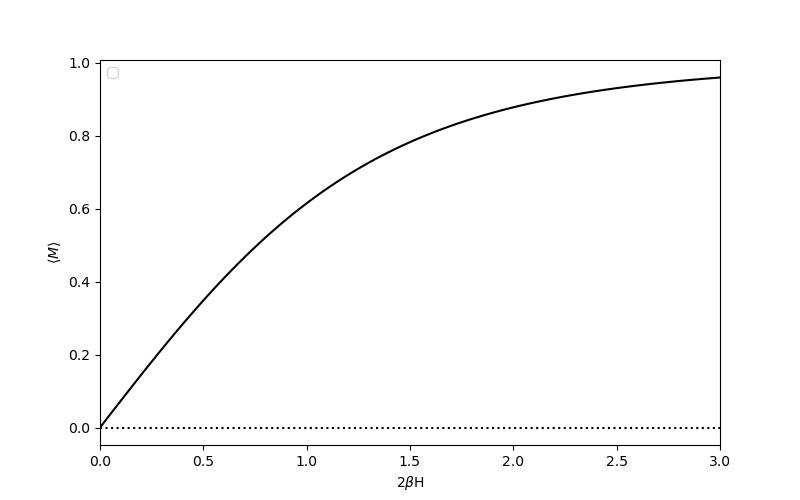
\includegraphics[width=100mm]{graph/fukushima(3_140).png}
    \caption{スピン期待値$\langle M \rangle$を$2\beta H$の関数としてプロット.ただし,$2\beta J = 1.0$に選んだ \label{fig:spin_graph} }
  \end{center}
\end{figure}

スピン期待値について,見方を変えた計算法を行う.分配関数(\ref{eq:分配関数})の最初の等号の定義式とスピン期待値(\ref{eq:スピン期待値})の最初の等号の定義式を見比べながら,$Z$を$H$で偏微分すると,
\begin{equation}
  \frac{\partial Z}{\partial H} = \beta \sum_{\sigma_1, \sigma_2}(\sigma_1 + \sigma_2)e^{-\beta E(\sigma_1, \sigma_2)} = 2\beta Z \langle M \rangle
\end{equation}
となることがわかる.これはよりコンパクトに
\begin{equation}
  \langle M \rangle = \frac{1}{2\beta} \frac{\partial}{\partial H} \ln{Z} \label{eq:コンパクトスピン期待値}
\end{equation}
と表すことができる.この関係式を使って,分配関数(\ref{eq:分配関数})の再右辺に与えた答えの表式から計算しても,式(\ref{eq:スピン期待値})と全く同じ$\langle M \rangle$が得られることを簡単に確かめられる.式(\ref{コンパクトスピン期待値})のような関係式は2スピン系に限らず一般に成り立つ.同様に$Z$の定義に立ち戻って考えると,$\beta$で偏微分すればエネルギー期待値が得られることがわかる,つまり
\begin{equation}
  \langle E \rangle = -\frac{\partial}{\partial \beta} \ln{Z} = \sum_{\bm{\sigma}} E(\bm{\sigma}) P(\bm{\sigma})
\end{equation}
が一般的に成り立つ.

\end{document}